\documentclass{standalone}
\usepackage{tikz}
\usetikzlibrary{calc}
\begin{document}

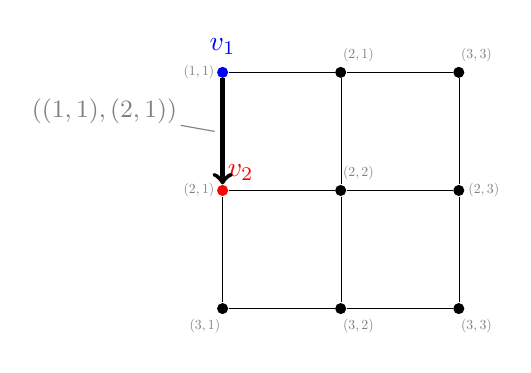
\begin{tikzpicture}[
  every node/.style={circle, fill=black, inner sep=1pt, minimum size=4pt}
]
  \node[label={[blue]above:$v_1$}] (a) at (0,3) [circle, color=blue] {};
  \node[draw=none, fill=none, scale=0.5, text=gray] (label2) at (-0.3,3) {$(1,1)$};
  \node[label={[red]above right:$v_2$}] (d) at (0,1.5) [circle, color=red] {};
  \node[draw=none, fill=none, scale=0.5, text=gray] (label2) at (-0.3,1.5) {$(2,1)$};
  \node[label={[gray, scale=0.5]above right:$(3,3)$}] (c) at (3,3) [circle, fill=black] {};
  \node[label={[gray, scale=0.5]above right:$(2,1)$}] (b) at (1.5,3) [circle, fill=black] {};
  \node[label={[gray, scale=0.5]above right:$(2,2)$}] (e) at (1.5,1.5) [circle, fill=black] {};
  \node[label={[gray, scale=0.5]right:$(2,3)$}] (f) at (3,1.5) [circle, fill=black] {};
  \node[label={[gray, scale=0.5]below left:$(3,1)$}] (g) at (0,0) [circle, fill=black] {};
  \node[label={[gray, scale=0.5]below right:$(3,2)$}] (h) at (1.5,0) [circle, fill=black] {};
  \node[label={[gray, scale=0.5]below right:$(3,3)$}] (i) at (3,0) [circle, fill=black] {};


  \node[draw=none, fill=none, font=\small, text=gray] (label1) at (-1.5,2.5) {$((1,1), (2,1))$};
  \draw[-, gray] (label1) -- (-0.1,2.25);
  
  \draw (a) edge[-, ultra thin](b);
  \draw (a) edge[->, ultra thick] (d);
  \draw (b) edge[-, ultra thin] (c);
  \draw (b) edge[-, ultra thin] (e);
  \draw (c) edge[-, ultra thin] (f);
  \draw (d) edge[-, ultra thin] (e);
  \draw (d) edge[-, ultra thin] (g);
  \draw (e) edge[-, ultra thin] (f);
  \draw (e) edge[-, ultra thin] (h);
  \draw (f) edge[-, ultra thin] (i);
  \draw (g) edge[-, ultra thin] (h);
  \draw (h) edge[-, ultra thin] (i);
\end{tikzpicture}

\end{document}
